\chapter{Phase Transitions}
\thispagestyle{empty}
\label{chap:phase_sec}

We have already introduced the ideas of measurement-induced phase transitions, and in this chapter, we provide a general overview of phase transitions. We briefly discuss classical phase transitions, and then, with the help of a simple model, we introduce the main tools, such as correlation functions, that we use in the coming chapters to analyze the MIPTs in a few different models.

\section{Classical Phase Transitions}

Classical phase transitions (CPTs) surround us in our everyday lives, and everyone has, at some point, experienced them firsthand. As we enjoy a drink on a hot summer day, we see the ice cubes melting and cooling down the glass. At atmospheric pressure, water freezes at $0^\circ C$ and boils at $100^\circ C$, and at these points, it undergoes a phase transition. Although everyone is familiar with these processes happening in everyday life, the physics behind them is quite interesting. Phase transitions are defined via discontinuities in the free energy derivatives with respect to thermal variables such as pressure or temperature. If we consider water, the quantity that shows drastic changes is the density. The density is proportional to the inverse of the volume, which in turn is related to the first derivative of the free energy with respect to pressure. An ice cube will float in a glass of water, so we know its density is lower than liquid water. If we heat ice, it will absorb heat, and its temperature will continuously rise until it has reached $0^\circ C$. At this point, the energy put into the system will not further heat the ice but will melt it. The energy needed to convert ice to liquid water at the critical temperature entirely is also known as \textit{latent heat}. Once all the ice has melted, it will continue to increase in temperature as more heat is added to the system until it reaches $100^\circ C$, where it will stop rising in temperature until the latent heat has wholly converted the liquid water into water vapor. At each of these points, while the temperature remains constant, the density changes, such that at atmospheric pressure and at $0^\circ C$ ($100^\circ C$), ice and liquid water (liquid water and vapor) have two densities. This discontinuity in the density defines these transition points, and as the discontinuity occurs in the first derivative of the free energy, these phase transitions involving latent heat are known as \textit{first-order} phase transitions. 

However, there are many more phases than just the ones we are familiar with in our everyday life. An iron magnet is ferromagnetic and produces a stable magnetic field; however, if heated to high enough temperatures, it undergoes a phase transition and becomes paramagnetic. To witness the transition, we typically choose an order parameter that exhibits distinct behavior in the two phases. For this example, magnetization is a useful order parameter. In the ferromagnetic phase, the spins are all aligned in the same direction, giving rise to non-zero total net magnetization. As the temperature increases, thermal fluctuations will start to destroy the ferromagnetic ordering, leading to a decrease in net magnetization. The magnetization will be zero at a critical temperature, and we enter the paramagnetic phase. Now, the spins randomly fluctuate around and have no preferred direction, and therefore, the net magnetization is zero at temperatures greater than the critical temperature. This is an example of a \textit{second-order phase transition}, or alternatively known as a \textit{continuous phase transition} due to the magnetization continuously decreasing to zero as the temperature increases and crosses the critical temperature. Another way of looking at this is by considering the symmetry present in the system. If we think about the direction rather than the magnitude of the magnetization vector, we see that this also allows us to characterize the phase transition as well. As mentioned before, the spins have no preferred direction at high temperatures, which is why the magnetization is zero. As no particular direction is preferred, we can describe this system as being rotationally invariant. Below the critical temperature, however, all spins are aligned in some direction, which means this rotational invariance of the system is no longer present, which is also known as spontaneous symmetry breaking.

More generally, symmetries are defined in symmetry groups, such as rotations or translations. For example, a two-dimensional rotation around an angle $\theta = 2 \pi/n$ generates the $\mathbb{Z}_n$ group. This describes the various symmetries that one encounters in nature, and the spontaneous breaking of symmetries is associated with phase transitions \cite{sachdev2011}. Furthermore, close to the critical point, the behavior of the order parameter can be investigated, and a critical exponent can be extracted. This exponent describes how the order parameter or a correlation function decays at criticality. Such critical exponents have been used to define universality classes, where the idea is that one can classify different types of transitions by their critical exponents \cite{odor2004}. Models belonging to a universality class do not necessarily exhibit the same behavior away from criticality; however, their behavior becomes increasingly similar close to it. 

\section{Quantum Phase Transitions}

After introducing some examples and features of phase transitions in general, let us now consider quantum phase transitions (QPTs)~\cite{sachdev2011, vojta2002, vojta2003,  heyl2018}. QPTs are phase transitions that occur in a quantum system at zero temperature. Hence, they do not occur as the result of tuning a thermal parameter but rather some other system parameter, such as a coupling term in the Hamiltonian. Therefore, thermal fluctuations cannot be the reason for quantum phase transitions to occur; instead, they are caused by quantum fluctuations. 

An example of a quantum phase transition can be seen in the transverse Ising model, where the Hamiltonian is defined by,
\begin{equation}
    \label{eq:transIsing}
    \hat{H} = -J \sum\limits_i \hat{\sigma}^z_i \hat{\sigma}^z_{i+1} - h \sum_i \hat{\sigma}^x_i,
\end{equation}

where $J$ is the interaction strength, $h$ the coupling strength of an external magnetic field in the $x$-direction, and $\hat{\sigma}^z_i, \hat{\sigma}^x_i$ are the Pauli matrices on site $i$. The transverse Ising model is the quantum equivalent of the classical Ising model. It is one of the simplest models exhibiting a quantum phase transition, allowing us to highlight the main concepts we use in later chapters to present measurement-induced phase transitions. In this section, we will focus on the quantum phase transition in $1D$. However, dynamical quantum phase transitions in this model in $2D$ have also been explored in recent years \cite{halimeh2017, hashizume2022}. Dynamical quantum phase transitions can occur when an initial state is prepared under a Hamiltonian with some initial control parameter, such as $h$ in Eq.~\ref{eq:transIsing} and then exploring the dynamics resulting from quenching the control parameter. Let us now explore some common tools used to highlight and explore quantum phase transitions in the $1D$ transverse Ising model.

The Transverse Ising Hamiltonian is invariant under flipping all spins in the $z$-direction. It is easy to verify that $\comm{\hat{H}}{\hat{P}} = 0$, where $\hat{P}$  is the spin-flip operator $\hat{P}  = \prod_i \hat{\sigma}^x_i$. A spin flip corresponds to a rotation about an angle $\theta = \pi$, which we mentioned earlier generates the $\mathbb{Z}_2$ group. As the Hamiltonian is invariant under this transformation, we say that it possesses a $\mathbb{Z}_2$ symmetry group. For the following analysis, we will consider $J = 1$ to define units of energy. 

A quantum system at absolute zero will be in its ground state, and without an external magnetic field ($h = 0$), the Hamiltonian exhibits two degenerate ground states, the two ferromagnetic states with all spins pointing either up ($\ket{\uparrow}$) or down ($\ket{\downarrow}$) in the $z$-direction. In reality, however, there is always a small external magnetic field that breaks this degeneracy, and the system favors one of these two states. Neither of these two states is invariant under the spin-flip operator, 
\begin{align}
\begin{split}
    \hat{P}  \ket{\uparrow} & = \ket{\downarrow} \\
    \hat{P}  \ket{\downarrow} & = \ket{\uparrow},
\end{split}
\end{align}
where $\ket{\uparrow}, \ket{\downarrow}$ are the two eigenstates of $\sigma_z$,
\begin{align}
\begin{split}
    \hat{\sigma}^z \ket{\uparrow} & = \ket{\uparrow} \\
    \hat{\sigma}^z \ket{\downarrow} & = - \ket{\downarrow}.
\end{split}
\end{align}

Then, as the coupling to the magnetic field $h$ is increased, there is a competition for the spins to all align (or anti-align) along the $z$ or the $x$ direction, which results in the order of the ferromagnetic ground state being destroyed. There are two degenerate ground states in the two limits $h = 0$ and $h \to \infty$. When choosing one ground state in a numerical simulation, one needs to select an eigenvector with the smallest eigenvalue. Due to the degeneracy, the chosen ground state will depend on the programming language or algorithm that is used in the simulation, leading to inconsistent results if we use the magnetization. For consistency, we therefore define an order parameter $P_{FM}$ given by the probability of finding the ground state in either one of the two ferromagnetic states, 
\begin{equation}
    P_{FM} = |\braket{\uparrow}{\psi}|^2 + |\braket{\downarrow}{\psi}|^2, 
\end{equation}
where $\ket{\psi}$ is the ground state that is found by the simulation. 

In Fig.~\ref{fig:Chapter1_Fig1}a), we see that for small $h$, the order parameter is $1$, indicating the ferromagnetic ordering of the ground state. As $h$ is increased, the ferromagnetic ordering of the ground state is destroyed, and the system undergoes a quantum phase transition at $h = 1$. In the limit $h \to \infty$ the ground state will point along the $x$-direction, where each spin will be in the superposition $\ket{\xrightarrow{}} = \frac{1}{\sqrt{2}}(\ket{\uparrow}+\ket{\downarrow})$. This state clearly is invariant under the spin-flip operator, $\hat{P}  \ket{\xrightarrow{}} = \ket{\xrightarrow{}}$. This phenomenon is known as spontaneous symmetry breaking. This phase transition is an example of a continuous phase transition, where the order parameter continuously changes with $h$, but the $\mathbb{Z}_2$-symmetry is broken. 

\begin{figure}[ht]
    \centering
    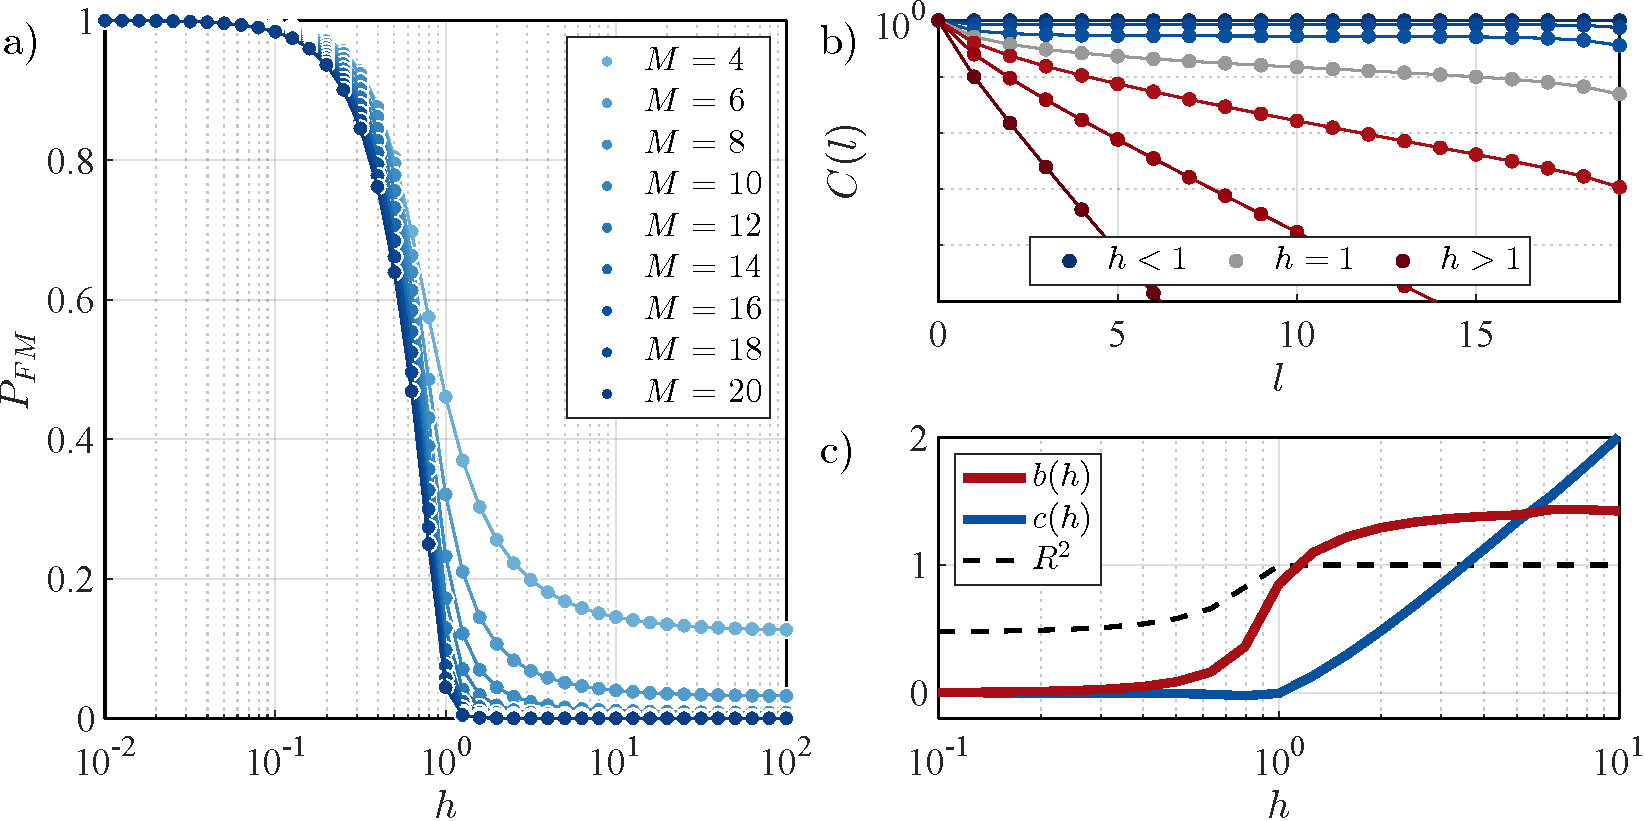
\includegraphics[width=\textwidth]{Chapters/Plots/Chapter2/Chapter1_Fig1.pdf}
    \caption{a) The ferromagnetic order parameter $P_{FM}$ as a function of the coupling strength $h$ of the external magnetic field for a range of system sizes. b) The correlation function $C(l) = \langle \hat{\sigma}^z_1 \hat{\sigma}^z_{1+l} \rangle$ for $M = 20$. c) The parameters of the fitting function $f(h) = a l^{-b} e^{-c l}$ used to fit the correlation function $C(l)$.} 
    \label{fig:Chapter1_Fig1}
\end{figure}

Correlation functions are another useful tool for investigating phase transitions; they are expectation values of products of operators that measure either temporal or spatial correlations. In the model we are considering, we define the correlation function $C(l) = \langle \hat{\sigma}^z_1 \hat{\sigma}^z_{1+l} \rangle$. For $h = 0$, it is easy to see that $C(l) = 1$ as the ferromagnetic ground state has long-range order \cite{carlin1986}. In the limit where $h \to \infty$, the correlation function will decay exponentially to $0$, i.e., $C(l) \propto \exp(- l/\xi)$, where $\xi$ is the length scale over which correlations decay. Typically, correlation functions near criticality exhibit algebraic decay with distance, and a correlation length $\xi$ that diverges \cite{carr2010}. To verify this, we consider the fitting function $f(h) = a l^{-b} \exp(-c l)$, and show the fitting parameters $b, c$ as a function of $h$ in Fig.~\ref{fig:Chapter1_Fig1}~c). The parameter $a$ is simply a scaling factor and does not offer additional insight in our analysis. For $h < 1$, the fit is not accurate ($R^2 \approx 0.5$), and the fitting function does not accurately describe the behavior of the correlation function. For $h \geq 1$, however, we have good agreement with the fitting function ($R^2 \approx 1$). At $h = 1$, we see that $c = 0$, i.e., the correlation function is purely characterized by the algebraically decaying term $l^{-b}$. As the correlation length $\xi$ is the inverse of the fitting parameter $c$, we see that if $c \to 0$, then $\xi \to \infty$. At the critical point, the correlation length diverges, and correlations are non-zero at all possible length scales; for infinite systems, the state and correlations at the transition point are said to be \textit{scale-invariant} \cite{carr2010, sachdev2011}. For $h > 1$, we see the value for $b$ saturates while $c$ continuously increases with $h$, indicative of the exponential decay taking over the behavior of the correlation function. It is important to note that, while $c=0$ also for $h<0$, and this is due to the bad fit for $h<1$. If we subtract the square of the magnetization $\expval{\hat\sigma^z}$, we would see that the correlation length $\xi$ only diverges at the critical point.

Everything we have seen here serves as an introduction to phase transitions and what we look for to determine their existence and behavior. The phase transitions we analyze in chapters~\ref{chap:MIPT_bosons}-\ref{chap:short_time_dynamics} have a different flavor; however, they result from local measurements in open quantum systems. Regardless, all the tools and characteristics we have seen here will be important as they allow us to characterize quantum phases similarly. Now, we continue with the introduction of open quantum systems and the numerical tools that will enable us to simulate them.